\documentclass{article}

\usepackage{fancyhdr}
\usepackage{extramarks}
\usepackage{amsmath}
\usepackage{amsthm}
\usepackage{amsfonts}
\usepackage{tikz}
\usepackage[plain]{algorithm}
\usepackage{algpseudocode}
\usepackage{siunitx}
\usepackage{hyperref}

\usetikzlibrary{automata, positioning}

%
% Basic Document Settings
%

\topmargin=-0.45in
\evensidemargin=0in
\oddsidemargin=0in
\textwidth=6.5in
\textheight=9.0in
\headsep=0.25in
\setlength{\parindent}{4em}
\setlength{\parskip}{1em}
\linespread{1.1}

\pagestyle{fancy}
\lhead{\hmwkAuthorName}
\chead{\hmwkClass\ Final Project }
\rhead{}
\lfoot{\lastxmark}
\cfoot{\thepage}

\renewcommand\headrulewidth{0.4pt}
\renewcommand\footrulewidth{0.4pt}

\setlength\parindent{1cm}
\def\BState{\State\hskip-\ALG@thistlm}

\graphicspath{{./figures/}}
%
% Create Problem Sections
%


\newcommand{\enterProblemHeader}[1]{
    \nobreak\extramarks{}{Problem \arabic{#1} continued on next page\ldots}\nobreak{}
    \nobreak\extramarks{Problem \arabic{#1} (continued)}{Problem \arabic{#1} continued on next page\ldots}\nobreak{}
}

\newcommand{\exitProblemHeader}[1]{
    \nobreak\extramarks{Problem \arabic{#1} (continued)}{Problem \arabic{#1} continued on next page\ldots}\nobreak{}
    \stepcounter{#1}
    \nobreak\extramarks{Problem \arabic{#1}}{}\nobreak{}
}

\setcounter{secnumdepth}{0}
\newcounter{partCounter}
\newcounter{homeworkProblemCounter}
\setcounter{homeworkProblemCounter}{1}
\nobreak\extramarks{Problem \arabic{homeworkProblemCounter}}{}\nobreak{}

%
% Homework Problem Environment
%
% This environment takes an optional argument. When given, it will adjust the
% problem counter. This is useful for when the problems given for your
% assignment aren't sequential. See the last 3 problems of this template for an
% example.
%
\newenvironment{homeworkProblem}[1][-1]{
    \ifnum#1>0
        \setcounter{homeworkProblemCounter}{#1}
    \fi
    \section{Problem \arabic{homeworkProblemCounter}}
    \setcounter{partCounter}{1}
    \enterProblemHeader{homeworkProblemCounter}
}{
    \exitProblemHeader{homeworkProblemCounter}
}

%
% Homework Details
%   - Title
%   - Due date
%   - Class
%   - Section/Time
%   - Instructor
%   - Author
%

\newcommand{\hmwkTitle}{Implementation and Analysis of a Real-Time Scientific Payload Control System}
\newcommand{\hmwkDueDate}{5/7/2018}
\newcommand{\hmwkClass}{COSC 6384}
\newcommand{\hmwkClassTime}{}
\newcommand{\hmwkClassInstructor}{Dr.Albert Cheng}
\newcommand{\hmwkAuthorName}{\textbf{Andrew G. Walker}}

%
% Title Page
%

\title{
    \vspace{2in}
    \textmd{\textbf{ \hmwkTitle}}\\
    \normalsize\vspace{0.1in}\small{Due\ on\ \hmwkDueDate\ at 3:10pm}\\
    \vspace{0.1in}\large{\textit{\hmwkClassInstructor\ \hmwkClassTime}}
    \vspace{3in}
}

\author{\hmwkAuthorName}
\date{}

\renewcommand{\part}[1]{\textbf{\large Part \Alph{partCounter}}\stepcounter{partCounter}\\}

%
% Various Helper Commands
%

% Useful for algorithms
\newcommand{\alg}[1]{\textsc{\bfseries \footnotesize #1}}

% For derivatives
\newcommand{\deriv}[1]{\frac{\mathrm{d}}{\mathrm{d}x} (#1)}

% For partial derivatives
\newcommand{\pderiv}[2]{\frac{\partial}{\partial #1} (#2)}

% Integral dx
\newcommand{\dx}{\mathrm{d}x}

% Alias for the Solution section header
\newcommand{\solution}{\textbf{\large Solution}}

% Probability commands: Expectation, Variance, Covariance, Bias
\newcommand{\E}{\mathrm{E}}
\newcommand{\Var}{\mathrm{Var}}
\newcommand{\Cov}{\mathrm{Cov}}
\newcommand{\Bias}{\mathrm{Bias}}

\begin{document}

\maketitle
\pagebreak
\tableofcontents
\pagebreak
\section{Introduction}


 Each year, NASA and the Louisiana Space Consortium graciously host payloads through the High Altitude Student Payload (HASP) program from students around the world on a high altitude balloon flight as a test bed for scientific and engineering projects. The harsh conditions in the stratosphere provide interesting engineering challenges and necessitate meticulous design and planning. Payloads must be designed to operate in near vacuum conditions with temperature fluctuations of up to \SI{80}{\celsius}. Additionally, payloads must be designed to operate on less than \SI{60}{\watt} of power and have the ability to operate autonomously in case of a communication failure. 
 
 
The Stratospheric Organism and Radiation Analyzer (SORA) payload from the University of Houston was accepted for the 2018 flight and should fly sometime in August. The purpose of this project was to apply techniques from real-time systems including scheduling and model checking to specify and implement a real system. In this report, the details of the specification and design of the SORA payload's control systems are presented as well as an analysis of the system's overall effectiveness.

\begin{figure}[H]
\centering
        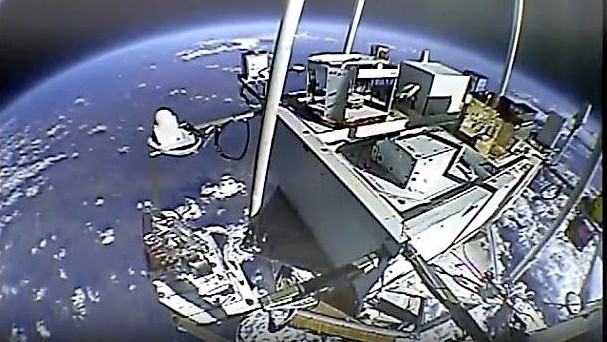
\includegraphics[scale=.5]{sora_flight.jpg}
    \caption{HASP gondola in the stratosphere.}
    \label{fig:flight}
\end{figure}
\pagebreak
\section{Design}
The SORA payloads main purpose is to sample for microorganisms present in the stratosphere using two modified diaphragm vacuum pumps and solenoids that can be opened and closed to seal collection chambers. The system will have 8 temperature sensors and two barometers to monitor the environmental conditions of the payload and the temperature of the pump system. The control system must be capable of monitoring environmental conditions and the health of the two pumps while accepting commands from ground control. It must also be able to ensure that if the conditions become unsuitable for collection or if the pumps become overheated the collection system is powered off and cannot be restarted until conditions return to normal. Specific constraints are listed below.

\begin{itemize}
\item Collection has to occur at or above \SI{26}{\kilo\meter}
\item Both pumps must maintain a temperature between \SI{0}{\celsius} and \SI{50}{\celsius}
\item Commands to start collection will only be accepted if the pumps are healthy and the payload is at the correct altitude
\item Commands to stop collection can be accepted at any time the system is in collection mode
\item The system should be able to respond to commands within \SI{50}{\milli\second}
\item If either the altitude is too low or the pumps are not at a healthy operating temperature the collection must be stopped and an error is raised
\end{itemize}

\begin{figure}[H]
\centering
        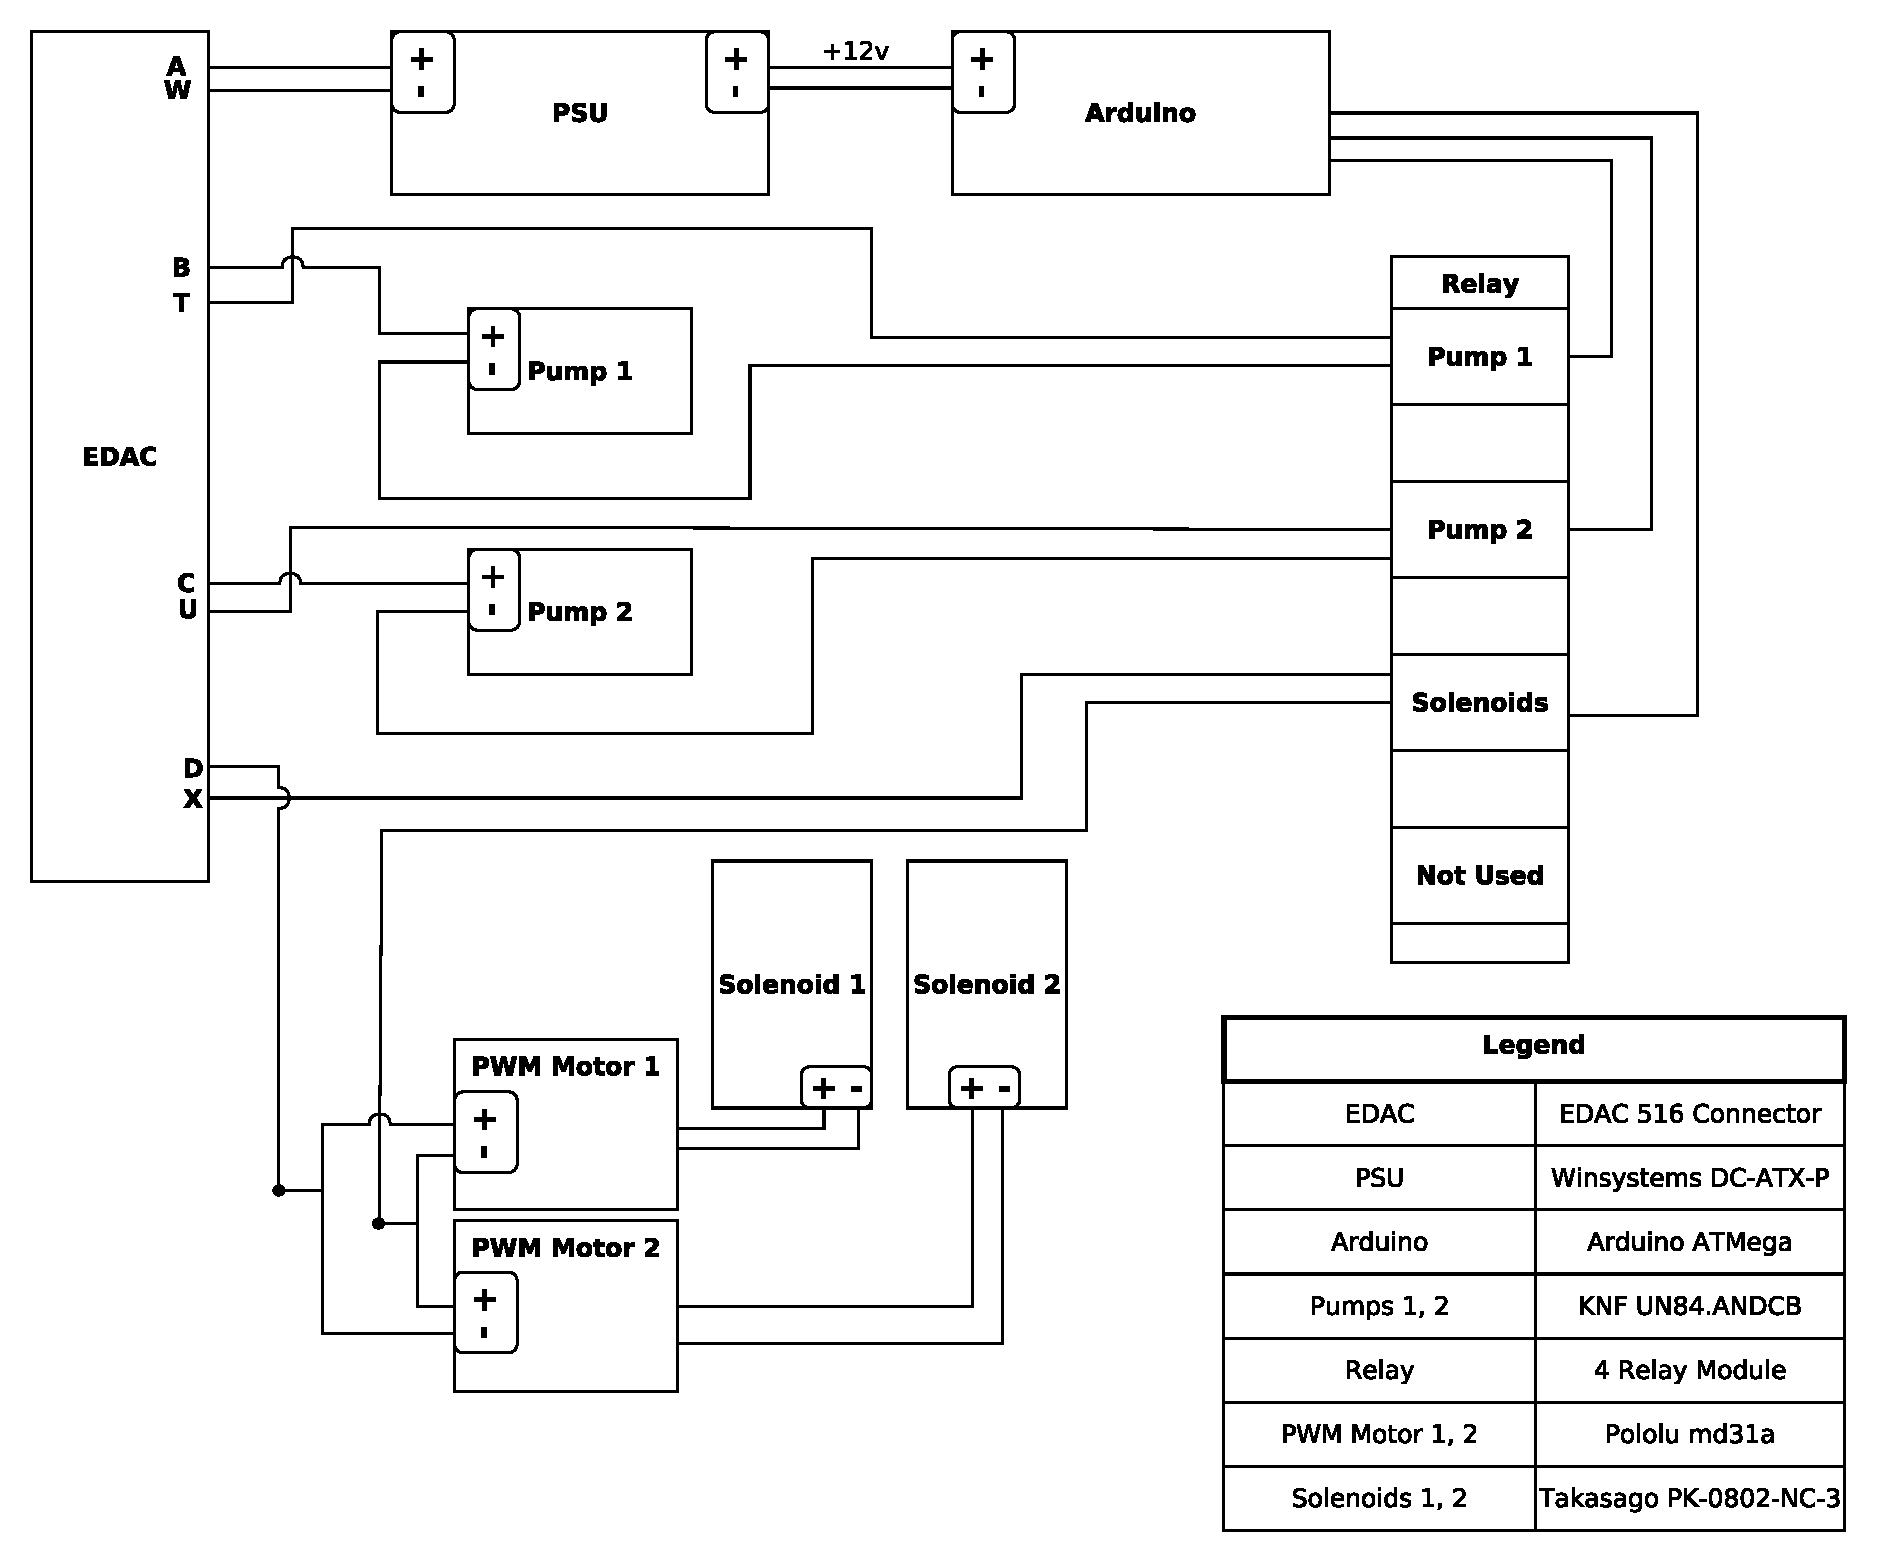
\includegraphics[scale=.25]{power-distro.pdf}
    \caption{Simple block diagram showing system design.}
    \label{fig:design}
\end{figure}

\subsection{Hardware}

The core hardware utilized for this project is the Arduino Mega 2560 R3, which is a development board base around the ATmega2560 microprocessor. The Arduino is a robust development board that provides 54 digital input and output pins, 16 analog pins, I2C interface and 4 separate hardware serial ports for interacting with various sensors and auxiliary components. The Atmega2560 operates at a clock rate of \SI{16}{\mega\hertz} and is used widely used for low power micro-controller applications.

An auxiliary board that sits on top of the main Arduino board will be utilized log sensor data and system messages. A relay board controlled by digital output pins is also utilized turn the pumps on and off. Commands from ground control are accepted via discrete commands and are first processed by digital logic and then fed into the Arduino as a simple low or high signal indicating whether a command is ready to be processed.

\begin{figure}[H]
\centering
        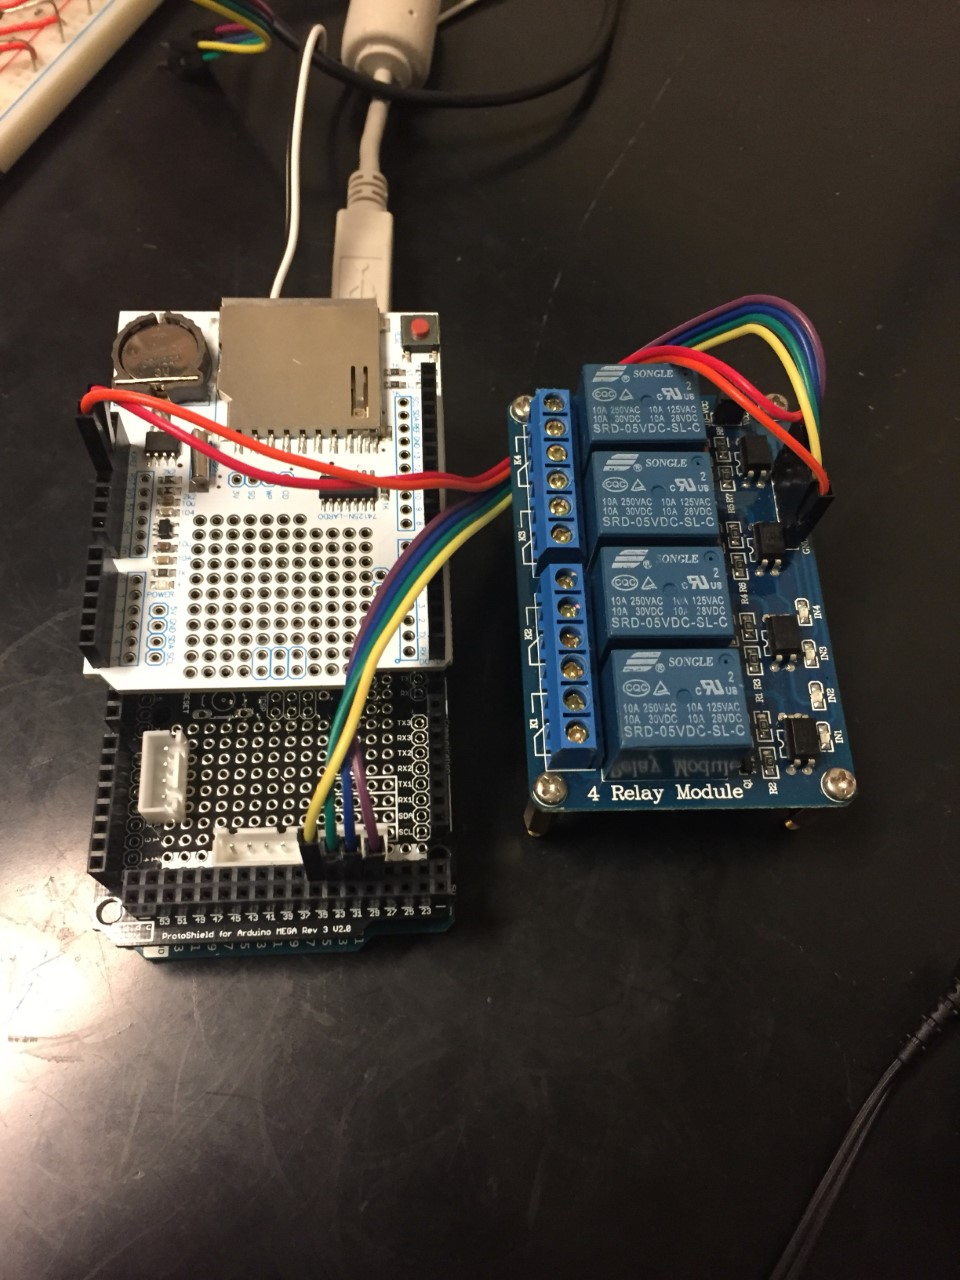
\includegraphics[scale=.25]{flight_computer.jpg}
    \caption{Arduino and accompanying data collection shield(left) and relay board(right).}
    \label{fig:flight}
\end{figure}

\subsection{FreeRTOS}

Unfortunately, the Atmega2560 and other processors in the AVR family are not supported by VxWorks as of yet. However, FreeRTOS is an open source real-time operating system that has been ported to a wide variety of hardware including the AVR family of microprocessors. In terms of functionality, FreeRTOS provides nearly all of the same features that VxWorks does, including priority based and round robin scheduling, built in support for semaphores and queues, hook facilities, and a robust faculty for tracing task execution.

\subsubsection{Overview}

FreeRTOS uses a static priority based scheduling algorithm that at every time instance selects the task with the highest priority to run. Other scheduling algorithms such as EDF and LLF have been implemented by various programmers in the open source community however they are not available by default and require an implementation for whatever specific hardware the system is running on.
\subsubsection{Tick System}
In any real time operating system it is imperative that the highest priority ready task be executing at any given point in time. Due to the discrete nature of microprocessors this is generally implemented as a system interrupt that happens at fixed intervals, wherein the scheduler interrupts the running task and determines whether to continue execution of that task or switch to a higher priority ready task. Specifically for the Arduino port of FreeRTOS, the on board watchdog timer is utilized to generate an interrupt at a user defined interval ranging from every \SI{15}{\milli\second} up to every \SI{500}{\milli\second}. Choosing the tick interrupt interval generally comes down to how responsive the system needs to be and how much time the processor will be idle. Short tick interrupts provide very fast system response for applications in which many different tasks will be preempting each other and a longer tick interrupt can be useful when sending the processor to sleep for long periods during CPU idle time. 
\begin{figure}[H]
\centering
        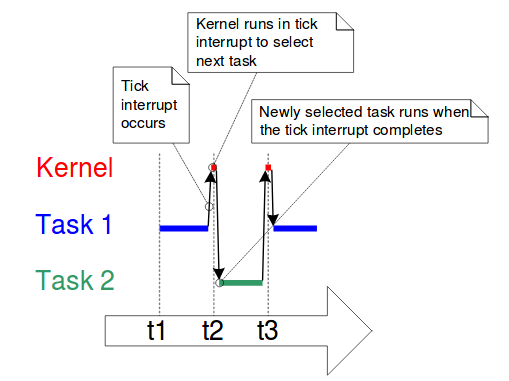
\includegraphics[scale=.5]{tick_interrupt.png}
    \caption{Demonstration of the kernel tick interrupt.}
    \label{fig:tick}
\end{figure}

\section{Model Checking}

A classical approach to modeling concurrent systems originally described by Clark et.al \cite{clark} is to specify them as a class of finite state automata referred to as a Kripke Structure. A Kripke Structure is composed of a set of states, atomic propositions true in each state and a set of binary relations between each state. One can then use a type of temporal logic called Computational Tree Logic (CTL) to prove various properties of the specified model. The Kripke structure corresponding to the SORA payloads specification and the propositions true in each state are shown in Figure \ref{fig:kripke} and  Table \ref{table:propositions} respectively. 

\begin{table}[H]
\begin{tabular}{ |l|c|c|c|c|c|c| }
\hline
 State & Pumps Running & Solenoids Engaged & Start CMD Received & Stop CMD Received & System Healthy&Error\\
\hline
$S_0$  & False & False & False & False & False& False \\ 
$S_1$  & False & False & False & False & True& False \\
$S_2$  & False & False & True & False & True& False \\
$S_3$  & False & True & True & False & True & False \\
$S_4$  & True & True & False & False & True & False \\
$S_5$  & False & True & False & False & False& True \\
$S_6$  & False & False & False & False & False& True \\
$S_7$  & False & True & False & True & True& False \\
 \hline
\end{tabular}
\caption{Table of atomic propositions true in each state.}
\label{table:propositions}

\end{table}
\begin{figure}[H]

\begin{center}
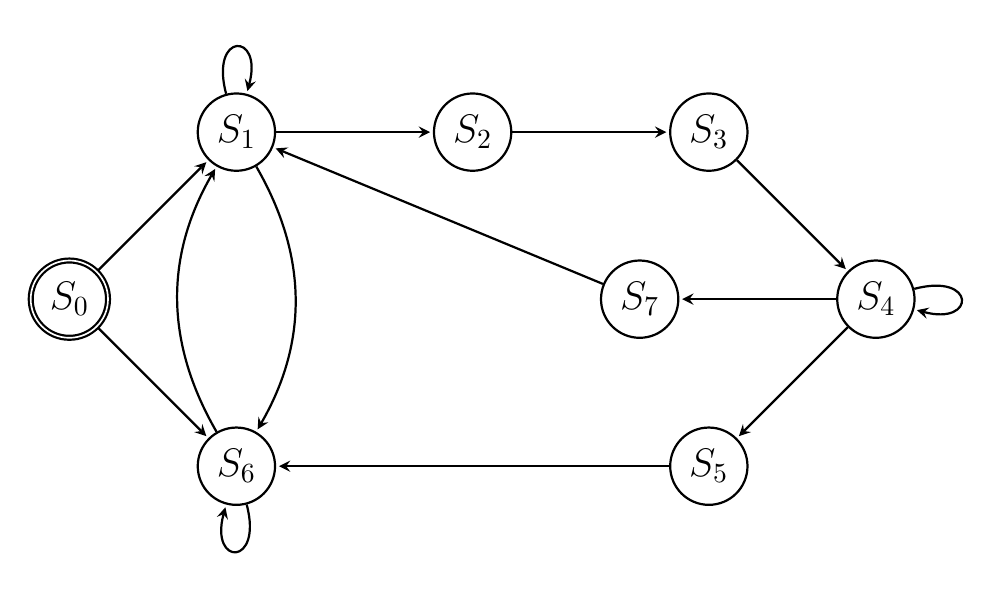
\begin{tikzpicture}[->,>=stealth,shorten >=1pt,auto,node distance=3cm,
                    thick,main node/.style={circle,draw,font=\sffamily\Large\bfseries}]

  \node[main node, accepting] (1) {$S_0$};
  \node[main node] (2) [below right of=1] {$S_6$};
  \node[main node] (3) [above right of=1] {$S_1$};
  \node[main node] (4) [right of=3] {$S_2$};
  \node[main node] (5) [right of=4] {$S_3$};
  \node[main node] (6) [below right of=5] {$S_4$};
  \node[main node] (7) [left of=6] {$S_7$};
  \node[main node] (8) [below left of=6] {$S_5$};


   \path[every node/.style={font=\sffamily\small}]
     (1) edge node [right] {} (3)
         edge node {} (2)
      (2) edge [bend left] node[right] {} (3)
      	  edge [loop below] node {} (2)
      (3) edge [bend left] node [left] {} (2)
      	  edge node {} (4)
          edge [loop above] node {} (3)
      (4) edge node [right] {} (5)
      (5) edge node [right] {} (6)
      (6) edge node [left] {} (7)
          edge node [left]  {} (8)
          edge [loop right] node {} (6)
      (7) edge node [left] {} (3)
      (8) edge node [left] {} (2);
%      (9) edge node [left] {} (10)
%      (10) edge node [left] {} (1);
\end{tikzpicture}
\end{center}
\caption{Representation of system specification as a Finite State Automata }
\label{fig:kripke}
\end{figure}


CTL can specify a set of logical constraints that must be satisfied by the the model. After defining the model in a modeling language a model checking tool can be used to explore the state graph and ensure that the CTL formula is satisfied. Using the SMV language \cite{smv} developed at Carnegie Mellon University, I was able to model the SORA control system and model check its safety assertions specified in CTL defined in Table \ref{table:logic}. A full description of the system in the SMV language is provided in Appendix A.
\begin{table}[H]
\begin{center}
\begin{tabular}{ |l|p{12cm}|}
\hline
\textbf{CTL Formula} & \textbf{English translation} \\
\hline
$AG(\neg e \cup \neg b)$ & Pumps will never be running when there's an error. \\
\hline
$AG(d \rightarrow AF(\neg a \wedge \neg b))$ & When the stop command is  received the pumps and solenoids eventually turn off.\\
\hline
$AG(\neg e \wedge a \rightarrow AF(\neg a \wedge \neg b))$ & When the system becomes unhealthy while running the pumps and solenoids eventually turn off.\\
\hline
$AG(c \wedge e\rightarrow AF(a \wedge b))$ & When the start command is received and the system is healthy the pumps and solenoids eventually turn on.\\
\hline
$AG(e \rightarrow AF(\neg a \wedge \neg b))$ & When the system becomes unhealthy the pumps and solenoids eventually turn off.\\
\hline

\end{tabular}
\caption{CTL formulas and their English translations.Note that the symbols a,b,c etc. correspond to the propositions defined in Table \ref{table:propositions} e.g a = "Pumps Running" b = "Solenoids Engaged" etc.}
\label{table:logic}
\end{center}
\end{table}
\subsection{Proving Correctness Using NuSMV}
Using the reimplementation of the SMV model checker NuSMV \cite{smv}, I was able to verify that the CTL specifications are satisfied by the model created in SMV. The output of the model checker, shown in Figure \ref{fig:output}, shows that all of the CTL specifications from Table \ref{table:logic} are true. An interesting feature of this model checker is that given a CTL specification that is not true, the model checker will provide a counter-example showing a series of state transitions that lead to a case where the formula is false. From the output one can see that the assertion which in English corresponds to, "If the start command is received all paths of execution eventually result in the pumps turning on" is determined to be false. The output then shows that in the case where the start command is received and the system is not healthy, the pumps will not be turned on and an error will be raised. A full graph representing all transition relations is shown in Figure \ref{fig:transitions}

\begin{figure}[H]
\centering
        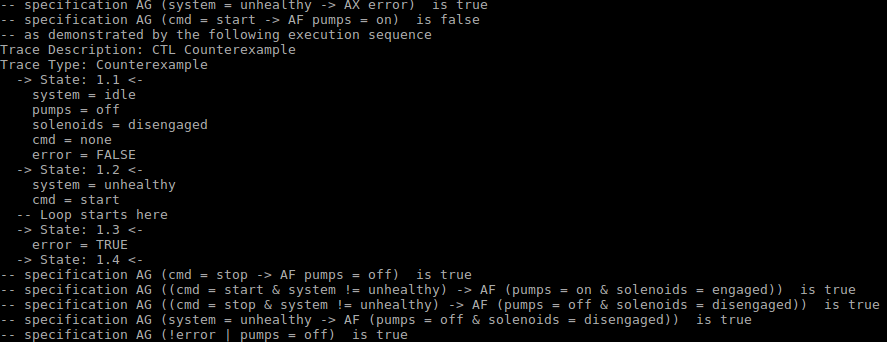
\includegraphics[scale=.5]{output.png}
\caption{Output of NuSMV specification verification}
    \label{fig:output}
\end{figure}

\begin{figure}[H]
\centering
        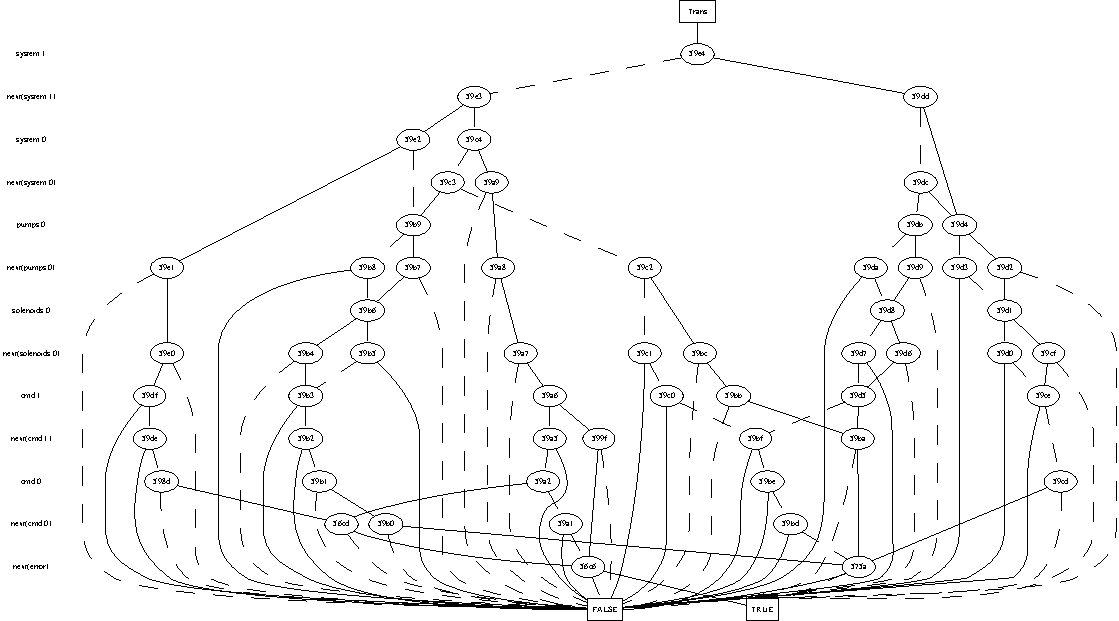
\includegraphics[scale=.9]{transitions-cropped.pdf}
    \caption{Graph generated by NuSMV that displays all transition relations.}
    \label{fig:transitions}
\end{figure}
\pagebreak
\section{Implementation}
\subsection{Designing a Feasible Task Set}
The task set is fairly simple and is composed of periodic and sporadic tasks. Tasks that monitor the temperature and pressure of the payload are modeled as periodic tasks that are executed every  \SI{25}{\milli\second} and \SI{30}{\milli\second} respectively. Tasks that monitor the health of the payload and check for new commands are modeled similarly with a period of \SI{50}{\milli\second}. Tasks that are performed in response to a command being received are modeled as sporadic tasks that can occur with a minimum separation of one period of the command checking task. The execution time of these sporadic tasks is accounted for in worst case execution time of the command monitoring task. Determining if the task set can be feasibly scheduled given the desired system response time of  \SI{50}{\milli\second} requires a priori knowledge of tasks start time, periods, and worst case execution time (WCET). 

\subsection{Determining WCET}
Determining the WCET of a task is not trivial and there are a wide variety of techniques for doing so. In general, techniques fall into two categories: measurement of the task execution times empirically or static analysis of a tasks actual instructions. For this project, I decided to use a simple measurement method. The Arduino has a built in timer accurate to \SI{4}{\micro\second} that was utilized in combination with kernel hooks provided by FreeRTOS to time the tasks while the system was in operation. The best case, worst case, average case and standard deviation of various for various system actions is shown in Table\ref{table:execution} and each tasks execution time in microseconds and period is displayed in Table \ref{table:tasks}.

\begin{table}[H]
\begin{center}
\begin{tabular}{ |l|c|c|c|c|}
\hline
\textbf{System Action} & \textbf{Best Case} & \textbf{Worst Case} & \textbf{Average Case} & \textbf{$\sigma$} \\
\hline
Temp. Read &  476 & 528 & 504.31 &3.44\\ 
Press. Read & 676 & 712 &  694.28 & 2.87\\
Punch Solenoid & 16  & 24 & 19.2 & 1.23\\
Hold Solenoid &  16 & 24 & 19.2 & 1.30\\
Disengage Solenoid & 16 & 24 & 19.4 & 1.20\\
Engage Pump & 4 & 16 & 6.71 & 1.12\\
Disengage Pump & 4 & 16 & 6.83 & 1.12\\
Command Monitor & 364 & 376 & 370.34 & 2.67\\
Health Monitor & 344 & 442 & 373.23 & 1.56\\
\hline

\end{tabular}
\caption{Execution time of tasks in \SI{}{\micro\second}}
\label{table:execution}
\end{center}
\end{table}.

\begin{table}[H]
\begin{center}
\begin{tabular}{ |l|c|c|c|c|}
\hline
\textbf{Task} & \textbf{Execution Time ($c_{i}$)
} & \textbf{Period ($p_{i}$)} \\
\hline
Temp. Read (x8) &  4224 & 25000\\ 
Press. Read (x2) & 1424 & 30000\\
Command Monitor & 376 & 50000 \\
Health Monitor & 442 & 50000 \\
\hline

\end{tabular}
\caption{Execution time and periods of tasks in \SI{}{\micro\second}}
\label{table:tasks}
\end{center}
\end{table}.

\subsection{Schedulability Analysis}
 Once WCET for each task is known it's fairly straight forward to determine if the task set is schedulable within the hyper period. By calculating the LCM of the task's periods one can determine that the hyper period for this task set is \SI{150}{\milli\second}. Then using the sufficient condition for RM schedulability outlined by Liu and Layland \cite{ll} 

\[
U \leq n(2^{\frac{1}{n}}-1)
\]

we can verify that

\[ U = \sum \frac{c_{i}}{p_{i}} = 0.208 \leq 4(2^{\frac{1}{4}}-1) \leq .7568\]

Since the condition is satisfied, we can see that the task set is schedulable and utilizes about 21\% of the available processing power. A lower bound on the system response time to commands can now be calculated by determining the minimum period for the command task such that task set is still schedulable. In order to determine this period we can use time demand analysis. In order for the task set to be RM schedulable it must satisfy the following inequalities


\[c_1 + c_2 + c_3 + c_4 \leq 25000 \]
\[2c_1 + c_2 + c_3 + c_4 \leq 30000 \]
\[2c_1 + 2c_2 + c_3 + c_4 \leq 50000\]

In order to determine the minimum value for the command monitor task's period we need to determine minimized $p_{3}$ that satisfies at least one of the following inequalities

\[c_1 + c_2 + c_3\left\lceil \frac{50000}{p_3}\right\rceil + c_4 \leq 25000 \]
\[2c_1 + c_2 + c_3\left\lceil \frac{50000}{p_3}\right\rceil + c_4 \leq 30000 \]
\[2c_1 + 2c_2 + c_3\left\lceil \frac{50000}{p_3}\right\rceil + c_4 \leq 50000\]
\pagebreak


Since only one inequality need to be satisfied we can choose the inequality with the largest right hand side and determine

\[c_3\left\lceil \frac{50000}{p_3}\right\rceil \leq 38262\]
\[\left\lceil \frac{50000}{p_3}\right\rceil \leq 101.76\]
\[p_3 \geq 493 \]

Thus, providing a lower bound on the period of the command task. This implies that theoretically the system could respond to commands within \SI{493}{\micro\second} without missing deadlines. After modifying the task set to have this new period, time demand analysis was performed on a computer to verify the result as shown in Figure \ref{fig:timedemand} 

    \begin{figure}[H]
\centering
        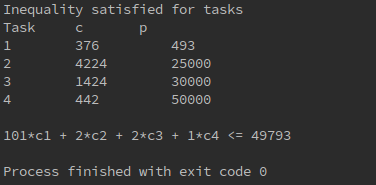
\includegraphics[scale=.75]{timedemand.png}
    \caption{Output from time demand analysis.}
    \label{fig:timedemand}
\end{figure}


\subsection{Leveraging the Idle Task for Saving Power}

Since the task set doesn't fully utilize the CPU, there will be a considerable amount of idle time where all tasks are either waiting or blocked. In FreeRTOS there must always exist a task that is ready to run, so at the time of scheduler initialization an idle task is always created with the lowest possible priority in the system. This idle task is then executed whenever no tasks are in the ready queue and can then be hooked into by the application developer. If the idle task is left unimplemented, it simply cycles in and out of the idle task wasting CPU cycles. An interesting use of this idle time in embedded applications is putting the system into a low power state in order to conserve energy. By using the idle task hook provided by FreeRTOS in combination with the built in sleep functionality of the ATmega2560, one can easily implement this functionality on an Arduino based system. However, the frequency of the tick interrupt can have a drastic affect on the amount of power saved using this method.

	Sleep mode on AVR based processors sends the processor into a low power state until an interrupt, either external or from a timer occurs. Since the watchdog timer initiates an interrupt at every tick, during idle periods the processor is sent to sleep and woken up each time a tick interrupt occurs. If the tick period is set too low then often the power saved by entering sleep mode is offset by the amount of overhead from context switching between the scheduler and the idle task as demonstrated in Figure~\ref{idleint}. This can of course be mitigated somewhat by lengthening the interval of the tick interrupt allowing the idle task to spend more time sleeping. However one must be careful to not set the tick interrupt too high as it could reduce system response time. I found that a good compromise between power savings and system response time for my specific application is around \SI{30}{\milli\second}.
    
    \begin{figure}[H]
\centering
        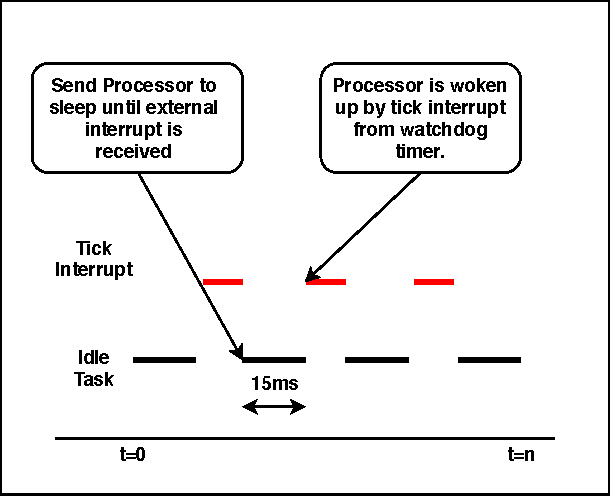
\includegraphics[scale=.75]{PreemptionDiagram.pdf}
    \caption{By default the idle task is interrupted by the tick interrupt at \SI{15}{\milli\second} intervals negating much of the power saving obtained by sending the CPU to sleep during idle periods.}
    \label{idleint}
\end{figure}



AVR based processors support a variety of low power modes that can be leveraged to save power. After implementing the idle task to send the system into a low power state I then measured the maximum, minimum and average power draw over a period of one minute for each of the provided low power modes as shown in table \ref{table:pwr}. With no sleep mode defined in the idle function the system draws around \SI{169}{\milli\ampere} but utilizing the various sleep modes provided by the system the power draw can be reduced to a minimum of around \SI{141}{\milli\ampere} providing a 16.57\% reduction in power draw. Note that the power draw measured here is from the entire board including the voltage regulator and on board status LEDs the actual power drawn from the CPU can be determined by subtracting the nominal current from the current draw when the CPU is shut down.
    
\begin{table}[H]
\begin{center}
\begin{tabular}{ |l|c|c|c|c|c| }
\hline
 Power Saving Mode & Min & Max & Avg. & Power Saved & \%\\
\hline
 Sleep Disabled & 0.168 & 0.170 & 0.169 & 0 & 0\\ 
 SLEEP\_MODE\_IDLE & 0.146 & 0.151 & 0.149 & 0.020&11.83 \\
 SLEEP\_MODE\_ADC & 0.147  & 0.149 &  0.147 & 0.022& 13.02\\
 SLEEP\_MODE\_POWER\_SAVE & 0.148 & 0.151 & 0.149 & 0.020&11.83  \\
 SLEEP\_MODE\_POWER\_STDBY & 0.142 & 0.145 & 0.142 & 0.027 & 15.98 \\
 SLEEP\_MODE\_POWER\_DOWN & 0.136 & 0.145 & 0.141 & 0.028 & 16.57 \\
 \hline
\end{tabular}
\end{center}
\caption{Comparison of different power modes}
\label{table:pwr}
\end{table}
\subsection{Power Saving}
 Sending the system into a low power state during the idle task is a fairly simplistic solution to saving power. Several techniques exist to solve this problem in a more elegant fashion, one of the most popular of which is Dynamic Voltage Scaling (DVS). DVS is a technique in which the clock speed and voltage of a CPU are scaled dynamically based on the slack time of a task set. Since the power function of a processor as it relates to clock speed is convex this generally creates very good power saving results. An example of an offline low power scheduling algorithm utilizing this technique was proposed by Yao et.al \cite{yao}.
 
 
While the Arduino board specifically does not support dynamic voltage scaling such a board could be developed and so it is interesting to explore how the idle shutdown method compares to a DVS technique. In the aforementioned paper an optimal scheduling algorithm was developed utilizing an intensity factor $g$ which calculates a lower bound on average processing speed for a set of tasks on an interval $[z, z^{'}]$. The algorithm identifies a critical region that maximizes $g$ and then schedules it on that interval before reseting the deadlines and arrival time of other tasks in that interval.

After running a simulation of this algorithm using the task set from Table \ref{table:tasks} it was determined that the entire task set can be scheduled with a $g$ value of 0.2096. Thus, we can run the CPU at roughly 21\% of its maximum speed of \SI{16}{\mega\hertz} and still meet deadlines. A feasible EDF schedule generated by the simulation is shown in Figure \ref{fig:schedule}. 
\begin{figure}[H]
\centering
        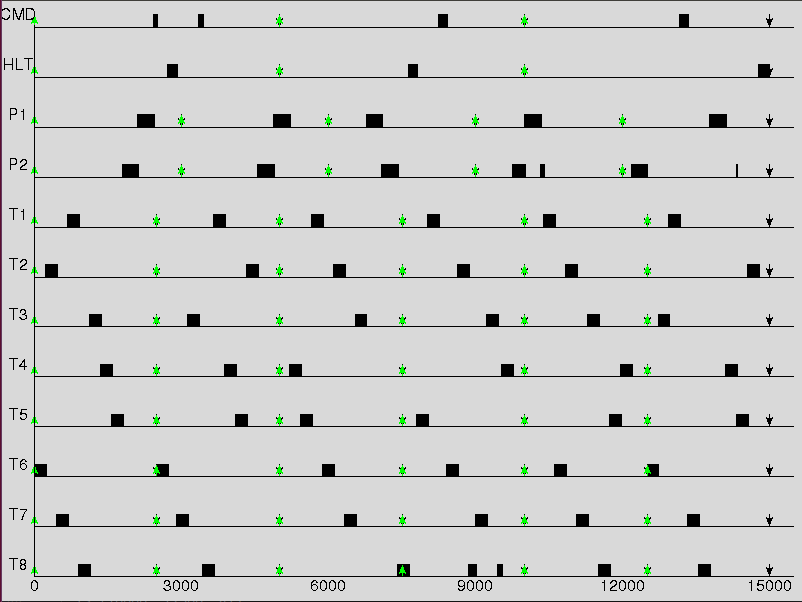
\includegraphics[scale=.4]{feasible_schedule.png}
    \caption{Feasible schedule for one hyper-period of \SI{150}{\milli\second} }
    \label{fig:schedule}
\end{figure}

Given that the task set can be feasibly scheduled at a much slower speed, it's interesting to explore what the actual performance would be at that speed. Shown in Figure \ref{pwrvfreq} is the power draw from the Atmega2560 as a function of processor speed. Running at 21\% of \SI{16}{\mega\hertz} at \SI{5}{\volt} shows a total power reduction of approximately \SI{17}{\milli\ampere} which is slightly lower than what was achieved by the idle shutdown technique. This difference is likely due to the fact that shutting down the CPU also turns off power hungry systems that are independent of the CPU clock speed such as the ADC. The graph only displays power saved specifically by the CPU and does not factor in many of the other components that could potentially be shutdown or slowed as well. This seems to imply that, for this specific application DVS would perform worst than the simple CPU idle shutdown method.
 
\begin{figure}[H]
\centering
        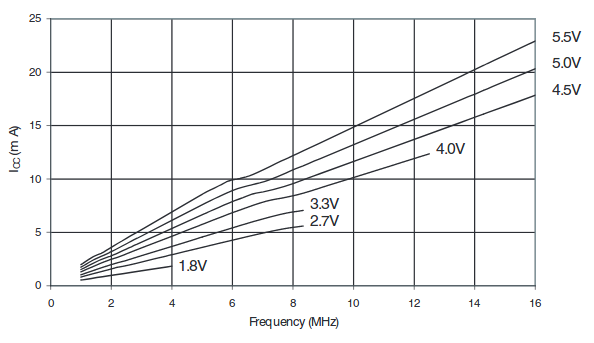
\includegraphics[scale=.75]{powervfrequecy.png}
    \caption{Active Supply Current Vs. Frequency from the Atmega2560\cite{2560datasheet} datasheet.}
    \label{pwrvfreq}
\end{figure}


\section{Conclusion}
Overall, the real-time systems techniques utilized proved to be very helpful for the specification and implementation of the controls systems for the SORA payload. The system specification was proven to be correct using model checking and CTL,  a theoretical lower bound on command response time of \SI{493}{\micro\second} was calculated and a 16\% power saving was achieved by using a simple idle shutdown technique. Finally, a theoretical calculation on the amount of power saved by slowing the clock speed shows that more power is saved by using a CPU shutdown technique which implies that it would likely not be beneficial to switch to a board that supports DVS.
\pagebreak
\begin{thebibliography}{1}
\bibitem{clark} 
Clarke, E. M., Emerson, E. A., \& Sistla, A. P. (1983). Automatic verification of finite state concurrent system using temporal logic specifications. Proceedings of the 10th ACM SIGACT-SIGPLAN Symposium on Principles of Programming Languages - POPL 83. doi:10.1145/567067.56708

\bibitem{smv}
NuSMV Reimplementation of the SMV Modeling Language at \href{http://nusmv.fbk.eu/}{http://nusmv.fbk.eu/}

\bibitem{2560datasheet}

Atmel Atmega 2560 datasheet: \href{http://ww1.microchip.com/downloads/en/DeviceDoc/Atmel-2549-8-bit-AVR-Microcontroller-ATmega640-1280-1281-2560-2561_datasheet.pdf}{\url{http://ww1.microchip.com/downloads/en/DeviceDoc/Atmel-2549-8-bit-AVR-Microcontroller-ATmega640-1280-1281-2560-2561_datasheet.pdf}}

\bibitem{yao}
Frances Yao, Alan Demers, Scott Shenker (1995).
A Scheduling Model for Reduced CPU Energy, Xerox Palo Alto Research Center

\bibitem{ll}
Liu, C. L.; Layland, J. (1973), "Scheduling algorithms for multiprogramming in a hard real-time environment", Journal of the ACM, 20 (1): 46–61, doi:10.1145/321738.321743
\end{thebibliography}

\pagebreak

\appendix
\section{Appendix A: Formal Specification in SMV}
\begin{verbatim}

MODULE main

VAR
    system: {executing, idle, unhealthy};
    pumps: {on, off};
    solenoids: {engaged, disengaged};
    cmd: {start, stop, none};
    error: boolean;
    

ASSIGN
    init(system) := idle;
    init(pumps) := off;
    init(cmd) := none;
    init(solenoids) := disengaged;

    next(system) :=
    case
	cmd = start & system != unhealthy: executing;
        cmd = stop & system != unhealthy: executing;
        cmd = none: {idle, unhealthy};
        TRUE: system;
    esac;

    next(pumps) :=
    case
	system = executing & cmd = start : on;
        system = executing & cmd = stop: off;
        system = unhealthy: off;
        TRUE: pumps;
    esac;

    next(solenoids) :=
    case
	system = executing & cmd = start : engaged;
        system = executing & cmd = stop: disengaged;
        system = unhealthy: disengaged;
        TRUE: solenoids;
    esac;

    next(cmd) :=
    case
	system = idle & next(system) != executing: {start, stop, none};
        TRUE: cmd;
    esac;

    next(error) :=
    case
	system = unhealthy: TRUE;
	system != unhealthy: FALSE;
    esac;

SPEC
AG(cmd = start & system != unhealthy -> AF(pumps = on & solenoids = engaged))

SPEC
AG(cmd = stop & system != unhealthy -> AF(pumps = off & solenoids = disengaged))

SPEC
AG(system = unhealthy -> AX(error));

SPEC

AG(system = unhealthy -> AF(pumps = off & solenoids = disengaged))

SPEC

AG(cmd = start -> AF(pumps = on));

SPEC

AG(cmd = stop -> AF(pumps = off));

SPEC

AG(!error | pumps = off);
\end{verbatim}

\end{document}
